%% FullCourse_10Lecs -- Lecture 4, Topic 4.4: Structured NNs + Accuracy/Validation
%% Source: ./archive_pre_split/Lec04_DL_RL_Macro.tex (sections 7-8)
%% Pass B: layer in M1_T4 ICNN/monotone refinements where applicable

%% Shared preamble for the FullCourse_10Lecs topic decks.
%%
%% Each topic .tex \input's this file, then defines its own \title, \date
%% override (if any), \graphicspath, and \begin{document}.
%%
%% Reconstructed verbatim from the inlined copy preserved in
%% Lec10_Case_Studies/Lec10_T8_Case6_DeepRamsey.tex (lines 23-190), which is
%% explicitly annotated there as "from ../shared_preamble.tex, copied verbatim".
%% Base preamble matches MiniCourse_8hr/Slides/shared_preamble.tex; this version
%% additionally provides \sectiondivider, the conceptbox/cautionbox/examplebox/
%% takeawaybox tcolorboxes, and \compacttables used across the split decks.

\documentclass[10pt,english,aspectratio=169]{beamer}

\usepackage{ae,aecompl}
\usepackage[T1]{fontenc}
\usepackage{textcomp}
\usepackage[utf8]{inputenc}
\usepackage{babel}
\usepackage{datetime2}

\setcounter{secnumdepth}{3}
\setcounter{tocdepth}{3}

\usepackage{amsmath, amssymb, amsthm, graphicx}
\usepackage{booktabs, multirow}
\usepackage{tikz}
\usepackage{pgfplots}
\pgfplotsset{compat=1.16}
\usepackage[most]{tcolorbox}
\tcbuselibrary{skins, breakable, theorems}
\usepackage{listings}
\usepackage{xcolor}

\lstset{
  basicstyle=\ttfamily\small,
  keywordstyle=\color{blue!80!black}\bfseries,
  commentstyle=\color{green!50!black}\itshape,
  stringstyle=\color{orange!80!black},
  backgroundcolor=\color{gray!8},
  frame=single,
  rulecolor=\color{gray!40},
  breaklines=true,
  showstringspaces=false,
  numbers=none,
}

\lstdefinestyle{pythonstyle}{
    language=Python,
    basicstyle=\ttfamily\footnotesize,
    keywordstyle=\color{blue!80!black}\bfseries,
    commentstyle=\color{green!50!black}\itshape,
    stringstyle=\color{orange!80!black},
    frame=single,
    breaklines=true,
    showstringspaces=false,
    numbers=left,
    numbersep=5pt,
    numberstyle=\tiny\color{gray},
    backgroundcolor=\color{gray!8},
    rulecolor=\color{gray!40}
}

\ifx\hypersetup\undefined
  \AtBeginDocument{%
    \hypersetup{bookmarks=false,breaklinks=true,pdfborder={0 0 0},colorlinks=true,
      linkcolor=DarkText,urlcolor=RedTitle}%
  }
\else
  \hypersetup{bookmarks=false,breaklinks=true,pdfborder={0 0 0},colorlinks=true,
    linkcolor=DarkText,urlcolor=RedTitle}%
\fi

\makeatletter
\newcommand\makebeamertitle{%
  \begin{frame}[plain]
    \vspace*{1.0cm}
    \centering
    {\usebeamerfont{title}\usebeamercolor[fg]{title}\inserttitle\par}
    \vspace{1.0cm}
    {\usebeamerfont{author}\usebeamercolor[fg]{author}\insertauthor\par}
    \vspace{0.2cm}
    {\usebeamerfont{date}\usebeamercolor[fg]{date}\insertdate\par}
  \end{frame}}%
\AtBeginDocument{%
  \let\origtableofcontents=\tableofcontents
  \def\tableofcontents{\@ifnextchar[{\origtableofcontents}{\gobbletableofcontents}}
  \def\gobbletableofcontents#1{\origtableofcontents}%
}

\usetheme{metropolis}
\usefonttheme{professionalfonts}

\definecolor{LightGray}{RGB}{230,230,230}
\definecolor{RedTitle}{RGB}{0,0,200}
\definecolor{VeryLightGray}{RGB}{245,245,245}
\definecolor{DarkText}{RGB}{0,0,0}

\setbeamercolor{background canvas}{bg=white}
\setbeamercolor{title}{fg=RedTitle}
\setbeamercolor{author}{fg=DarkText}
\setbeamercolor{date}{fg=DarkText}
\setbeamercolor{frametitle}{bg=VeryLightGray,fg=DarkText}
\setbeamercolor{normal text}{fg=DarkText}
\setbeamerfont{title}{size=\large}

\setbeamersize{text margin left=5mm, text margin right=5mm}
\addtobeamertemplate{frametitle}{}{\vspace{-0.5em}}
\newcommand{\reducevspace}{\vspace{-0.5cm}}

% Shared section divider and box styles for split topic decks.
\newcommand{\sectiondivider}[2]{%
\begin{frame}[plain,noframenumbering]
\begin{center}
\vfill
{\Large\textbf{#1}\par}
\vspace{0.35cm}
{\normalsize #2\par}
\vfill
\end{center}
\end{frame}
}

\newtcolorbox{conceptbox}[1][]{
  colback=blue!3,
  colframe=RedTitle!55,
  boxrule=0.35mm,
  arc=1mm,
  left=2mm,
  right=2mm,
  top=1mm,
  bottom=1mm,
  #1
}
\newtcolorbox{cautionbox}[1][]{
  colback=red!3,
  colframe=red!50!black,
  boxrule=0.35mm,
  arc=1mm,
  left=2mm,
  right=2mm,
  top=1mm,
  bottom=1mm,
  #1
}
\newtcolorbox{examplebox}[1][]{
  colback=green!3,
  colframe=green!45!black,
  boxrule=0.35mm,
  arc=1mm,
  left=2mm,
  right=2mm,
  top=1mm,
  bottom=1mm,
  #1
}
\newtcolorbox{takeawaybox}[1][]{
  colback=VeryLightGray,
  colframe=RedTitle!55,
  boxrule=0.35mm,
  arc=1mm,
  left=2mm,
  right=2mm,
  top=1mm,
  bottom=1mm,
  #1
}
\newcommand{\compacttables}{\renewcommand{\arraystretch}{1.15}}

\setbeamertemplate{navigation symbols}{}
\setbeamertemplate{footline}{%
  \hfill%
  \usebeamercolor[fg]{page number in head/foot}%
  \usebeamerfont{page number in head/foot}%
  \insertframenumber\,/\,\inserttotalframenumber\kern1em\vskip2pt%
}

\makeatother

\author{Zhigang Feng}
% "date with time": compile timestamp so each build is identifiable.
\date{\today\ \DTMcurrenttime}


\graphicspath{{./pic/}{../../MiniCourse_8hr/Slides/Module1_ML_Foundations/pic/}{../../MiniCourse_8hr/Slides/Module2_DL_RL_Macro/pic/}{../}}

% Suppress the redundant auto-generated metropolis section page; the
% \sectiondivider frames below are the dividers we keep.
\metroset{sectionpage=none}
\usetikzlibrary{positioning,arrows.meta,shapes,calc}
%% Lec04 shared MAP slide: "one map, four acts" recurring diagram.
%% Input this file AFTER ../shared_preamble.tex (needs RedTitle, VeryLightGray,
%% DarkText) and AFTER \usetikzlibrary{positioning,arrows.meta,shapes,calc}.
%% Call \LecFourMap{k} inside a frame, where k in {1,2,3,4} highlights the
%% current act ("you are here") and k = 0 renders the closing reprise with all
%% four acts checked green (used by T4's closing frame).
%% Filename deliberately does NOT match the build glob Lec*_T*.tex, so the build
%% script never tries to compile it standalone.
%%
%% The four acts are the lecture's story: PROBLEM -> SOLVE -> CODE -> TRUST,
%% one running example throughout (the optimal growth model): why grids break,
%% the Bellman route (deep VFI + actor-critic), the Euler route in PyTorch,
%% and structured networks + the validation gate.

\newcommand{\LecFourMap}[1]{%
% Precompute per-box style selectors; TikZ option lists are comma-split before
% TeX conditionals run, so \ifnum must not sit inside a [...] options list.
\ifnum#1=0
  \tikzset{lmapa/.style={lmapdone}, lmapb/.style={lmapdone},
           lmapc/.style={lmapdone}, lmapd/.style={lmapdone}}%
\else
  \tikzset{lmapa/.style={}, lmapb/.style={}, lmapc/.style={}, lmapd/.style={}}%
  \ifnum#1=1 \tikzset{lmapa/.style={lmapcur}}\fi
  \ifnum#1=2 \tikzset{lmapb/.style={lmapcur}}\fi
  \ifnum#1=3 \tikzset{lmapc/.style={lmapcur}}\fi
  \ifnum#1=4 \tikzset{lmapd/.style={lmapcur}}\fi
\fi
\begin{center}
\begin{tikzpicture}[
    act/.style={rectangle, rounded corners, draw=black!60, fill=VeryLightGray,
        minimum width=3.0cm, minimum height=0.95cm, text width=2.9cm,
        align=center, font=\small, text=DarkText},
    lmapcur/.style={draw=RedTitle, very thick, fill=orange!20},
    lmapdone/.style={draw=green!45!black, thick, fill=green!10},
    q/.style={font=\tiny\itshape, text width=3.0cm, align=center, text=black!70},
    barlab/.style={font=\tiny\bfseries, text=black!65},
    sat/.style={rectangle, rounded corners, draw=black!45, dashed, fill=white,
        text width=5.2cm, align=center, font=\tiny, text=black!70,
        minimum height=0.5cm},
    arr/.style={-{Stealth[length=2.2mm]}, thick, gray!60}
]
    % --- four act boxes ---
    \node[act, lmapa] (a1) at (0,0)
        {\textbf{4.1\ \ PROBLEM}\\[1pt] \tiny growth model $\cdot$ curse of dim.};
    \node[act, lmapb] (a2) at (3.6,0)
        {\textbf{4.2\ \ SOLVE}\\[1pt] \tiny deep VFI $\cdot$ actor--critic};
    \node[act, lmapc] (a3) at (7.2,0)
        {\textbf{4.3\ \ CODE}\\[1pt] \tiny Euler loss $\cdot$ PyTorch};
    \node[act, lmapd] (a4) at (10.8,0)
        {\textbf{4.4\ \ TRUST}\\[1pt] \tiny ICNN $\cdot$ validation $\cdot$ lab};
    \draw[arr] (a1) -- (a2);
    \draw[arr] (a2) -- (a3);
    \draw[arr] (a3) -- (a4);
    % --- the student question each act answers ---
    \node[q] at (0,-0.95)    {why do grids break on\\ real macro models?};
    \node[q] at (3.6,-0.95)  {how do neural nets solve\\ the Bellman equation?};
    \node[q] at (7.2,-0.95)  {how do I code it --- loss,\\ networks, training loop?};
    \node[q] at (10.8,-0.95) {can I trust the answer ---\\ and how do I prove it?};
    % --- "you are here" marker above the current act ---
    \ifnum#1=1 \node[font=\scriptsize\bfseries, text=RedTitle] at (0,0.98)
        {you are here\ $\blacktriangledown$};\fi
    \ifnum#1=2 \node[font=\scriptsize\bfseries, text=RedTitle] at (3.6,0.98)
        {you are here\ $\blacktriangledown$};\fi
    \ifnum#1=3 \node[font=\scriptsize\bfseries, text=RedTitle] at (7.2,0.98)
        {you are here\ $\blacktriangledown$};\fi
    \ifnum#1=4 \node[font=\scriptsize\bfseries, text=RedTitle] at (10.8,0.98)
        {you are here\ $\blacktriangledown$};\fi
    \ifnum#1=0 \node[font=\scriptsize\bfseries, text=green!45!black] at (5.4,0.98)
        {all four acts complete};\fi
    % --- bottom band: two solution routes + the audit (the technical spine) ---
    \fill[blue!10]   (-1.55,-1.72) rectangle (5.15,-1.40);
    \fill[green!12]  (5.65,-1.72)  rectangle (8.75,-1.40);
    \fill[orange!16] (9.25,-1.72)  rectangle (12.35,-1.40);
    \node[barlab] at (1.8,-1.56)  {BELLMAN ROUTE\ ($V$, $g$ networks)};
    \node[barlab] at (7.2,-1.56)  {EULER ROUTE\ (FOC residuals)};
    \node[barlab] at (10.8,-1.56) {AUDIT GATE\ (Lab 3A/3B)};
    % --- dashed satellites: where this lecture sits in the course flow ---
    \node[sat] at (1.5,-2.42)
        {\textit{upstream:} Lec03 --- the NN toolkit (architecture, UAT, training, ICNN)};
    \node[sat] at (9.3,-2.42)
        {\textit{downstream:} Lec05 --- the RL theory behind actor--critic; Lec06 --- heterogeneous agents at scale};
\end{tikzpicture}
\end{center}
}


\title[AI for Econ Research]{AI for Economic Research: Dynamic Models, Language, and Agents\\
Lecture 4.4: Structured NNs for Equilibrium \& Accuracy Validation}

\begin{document}

\makebeamertitle

%=============================================================================
\begin{frame}{Lecture 4 in One Map}
\textbf{One lecture, four decks, one running example: solve the optimal growth model with deep learning --- pose the problem, solve it two ways, code it, and prove the answer right.}

\LecFourMap{4}

\vspace{0.05cm}
\footnotesize\textit{\textbf{Act 4.4 (here)} earns the trust: inject concavity and monotonicity into the architecture (ICNN, monotone networks), then validate --- Euler-residual diagnostics and the Lab 3A/3B audit gate.}
\end{frame}

%=============================================================================
\section{Structured Neural Networks for Equilibrium Models}

\sectiondivider{Structured Neural Networks for Equilibrium Models}{ICNN and monotone networks: theory-consistent by construction}

%---------------------------------------
\begin{frame}{The Computational Challenge in Quantitative Macro}
\begin{itemize}
  \item \textbf{Nested ``Russian Doll'' structure}: Quantitative macro models involve \emph{multiple} nested optimization problems
  \medskip
  \item \textbf{Typical hierarchy}:
    \begin{enumerate}
      \item \textbf{Outer Loop}: Market clearing / calibration (solve for prices $p^*$)
      \item \textbf{Middle Loop}: Value function iteration (solve Bellman equations)
      \item \textbf{Inner Loop}: Agent optimization (choose $c, \ell, k'$ given state and prices)
    \end{enumerate}
  \medskip
  \item \textbf{Problem with unstructured nets}: Approximating value functions or costs with generic FFNNs turns the \emph{inner} problem into a non-convex optimization
    \begin{itemize}
      \item Multiple local optima and unstable outer iterations
      \item Economic misspecification (e.g., upward-sloping demand, non-concave value functions)
    \end{itemize}
\end{itemize}
\end{frame}

%---------------------------------------
\begin{frame}{Idea: Inject Economic Structure into the Network}
\textbf{Key idea}: Design architectures that \emph{respect} economic shape restrictions \emph{by construction}.

\vspace{0.3cm}
\centering
\begin{table}[]
\renewcommand{\arraystretch}{1.4}
\begin{tabular}{l | l | l}
\textbf{Property} & \textbf{Mathematical Gain} & \textbf{Economic Payoff} \\
\hline
\textbf{Convexity / Concavity} & Unique global optimum & Stable policy rules / VFI \\
\hline
\textbf{Monotonicity} & Invertible mappings & Well-behaved supply/demand \\
\hline
\textbf{Homogeneity} & $f(\lambda x) = \lambda f(x)$ & Consistency with balanced growth \\
\end{tabular}
\end{table}

\vspace{0.3cm}
\begin{itemize}
  \item This turns the neural net from a \textbf{black box} into a \textbf{glass box}: flexible enough to fit data, but disciplined by theory
\end{itemize}
\end{frame}

%---------------------------------------
\begin{frame}{Baseline: Standard Feed-Forward Networks}
\textbf{Generic FFNN architecture}:
\begin{itemize}
  \item Composition of affine maps and nonlinearities:
    \[
      y = f_\theta(x) = W_L\, \sigma\bigl(\ldots \sigma(W_1 x + b_1)\bigr)
    \]
  \item Layer weights $W^{(l)} \in \mathbb{R}^{d_l \times d_{l-1}}$ are \textbf{unconstrained}
\end{itemize}

\vspace{0.2cm}
\textbf{The optimization trap}:
\begin{itemize}
  \item Even if the \emph{true} value function is concave, the FFNN approximation generally is not
  \item When agents optimize against this approximation:
    \begin{itemize}
      \item FOCs are necessary but not sufficient
      \item Numerical solvers can converge to spurious local optima
      \item Comparative statics and equilibrium mappings can be erratic
    \end{itemize}
  \medskip
  \item \textbf{Solution}: Constrain the network architecture to guarantee the desired shape
\end{itemize}
\end{frame}

%---------------------------------------
\begin{frame}{Input Convex Neural Networks (ICNN)}
\textit{\footnotesize Amos, Xu \& Kolter (2017, ICML), ``Input Convex Neural Networks.''}
\textit{Recall:} the ICNN architecture and the convexity proof are introduced in Lec03 T4 (canonical foundations). Here we keep them only as much as needed and focus on the \emph{macro} application --- Lab 3A (classical ground truth) and Lab 3B (NN solution validated by Euler residual).

\vspace{0.2cm}
\textbf{Goal}: Construct $f(x)$ that is convex in $x$ \emph{by design}.

\vspace{0.2cm}
\textbf{Recursive definition}:
\[
  z_{l+1} = \sigma_l\left(\sum_{i=0}^l W_{l,i}^{(z)} z_i + W_l^{(x)} x + b_l\right)
\]

\textbf{Sufficient conditions for convexity}:
\begin{enumerate}
  \item \textbf{Non-negative recurrent weights}: all $W_{l,i}^{(z)} \geq 0$
  \item \textbf{Convex, non-decreasing activations}: $\sigma_l$ is convex and non-decreasing (e.g., ReLU, Softplus)
\end{enumerate}

\textbf{Result}:
\begin{itemize}
  \item $f(x)$ is convex in $x$ as a composition of convex, non-decreasing functions
  \item \textbf{Crucially}: Direct input weights $W_l^{(x)}$ can be \textbf{unconstrained} (including negative)
  \item This allows the network to learn the linear placement and slope freely
\end{itemize}
\end{frame}

%---------------------------------------
\begin{frame}{Why Impose Convexity in Macro?}
\small
Using ICNNs for value functions $V$ or pricing kernels delivers three benefits:

\begin{enumerate}
  \item \textbf{Robust Value Function Iteration}
    \begin{itemize}
      \item We solve $\max_{x'}\{u(x,x') + \beta\, \hat{V}(x')\}$
      \item If $\hat{V}$ is concave (or $-\hat{V}$ convex via ICNN), the objective is globally concave
      \item Fast, gradient-based \emph{convex} optimization with no local-maxima issues
    \end{itemize}

  \item \textbf{Well-Behaved Equilibrium Prices}
    \begin{itemize}
      \item Convex preferences $\Rightarrow$ monotone demand
      \item Unique, stable market-clearing price vectors
    \end{itemize}

  \item \textbf{Scalability to High Dimensions}
    \begin{itemize}
      \item ICNNs scale to high-dimensional state spaces while retaining the structure needed for Bellman contractions
    \end{itemize}
\end{enumerate}
\end{frame}

%---------------------------------------
\begin{frame}{ICNN: Proof Sketch (Why It's Convex)}
We prove by induction that each $z_l(x)$ is convex in $x$.

\vspace{0.2cm}
\textbf{Step 1: Base Case}
\begin{itemize}
  \item $z_0(x) = x$ is linear, hence convex \checkmark
\end{itemize}

\vspace{0.2cm}
\textbf{Step 2: Inductive Step}
\[
  z_{l+1}(x) = \sigma\bigl(W_z^{(l)} z_l(x) + W_x^{(l)} x + b_l\bigr)
\]
\begin{itemize}
  \item By induction, $z_l(x)$ is convex
  \item With $W_z^{(l)} \geq 0$: $W_z^{(l)} z_l(x)$ is a non-negative sum of convex functions $\Rightarrow$ convex
  \item Adding linear term $W_x^{(l)} x + b_l$ preserves convexity
  \item Applying convex, non-decreasing $\sigma(\cdot)$ to a convex argument preserves convexity \checkmark
\end{itemize}

\vspace{0.15cm}
\textbf{Therefore}: All layers $z_l(x)$, and hence $f(x)$, are convex in $x$
\end{frame}


%---------------------------------------
\begin{frame}{Do Constraints Limit Expressivity?}
\textbf{The concern}: By restricting $W_z \geq 0$, do we lose the universal approximation property?

\vspace{0.3cm}
\textbf{Theorem} (Chen, Shi \& Zhang, 2019, ICLR, ``Optimal Control Via Neural Networks: A Convex Approach''):
\begin{quote}
An Input Convex Neural Network can approximate \emph{any} convex function over a compact domain to arbitrary accuracy.
\end{quote}

\vspace{0.2cm}
\textbf{Intuition}:
\begin{itemize}
  \item A maximum of affine functions ($\max_i\{a_i^\top x + b_i\}$) is convex and can approximate any convex shape
  \item An ICNN with ReLU activations acts as a hierarchical max-affine approximator
\end{itemize}

\textbf{Implication for macro}:
\begin{itemize}
  \item You are not imposing a specific parametric form (like CES or Cobb-Douglas)
  \item You are imposing a \textbf{shape restriction} (convexity) while retaining non-parametric flexibility
\end{itemize}
\end{frame}

%---------------------------------------
\begin{frame}{Expressivity: The Economic Interpretation}
\textbf{Implication for macro}:
\begin{itemize}
  \item You are not imposing a specific parametric form (like CES or Cobb-Douglas)
  \medskip
  \item You are imposing a \textbf{shape restriction} (convexity) while retaining non-parametric flexibility
  \medskip
  \item This is useful when theory tells us the global shape, but not the exact curvature
\end{itemize}

\bigskip
\begin{center}
\textit{Architecture encodes theory; the data still choose the function inside that theory-consistent class.}
\end{center}
\end{frame}

%---------------------------------------
\begin{frame}{Partial Convexity: The Macro Reality}
\textbf{The issue}: Value functions $V(k, z)$ are typically:
\begin{itemize}
  \item \textbf{Concave} in endogenous states $k$ (capital, assets)
  \item \textbf{Non-concave / arbitrary} in exogenous states $z$ (TFP, income shocks)
\end{itemize}
A standard ICNN would incorrectly enforce convexity on $z$ as well.

\vspace{0.3cm}
\textbf{The solution: Partial ICNN (PICNN)}

Modify the architecture to distinguish between convex inputs ($u$) and non-convex inputs ($v$):
\[
  z_{l+1} = \sigma\left(\underbrace{W_z^{(l)} z_l}_{\geq 0} + \underbrace{W_u^{(l)}(u \circ v)}_{\text{interaction}} + \underbrace{W_v^{(l)} v}_{\text{free}} + b_l\right)
\]

\textbf{Implementation}: Pass $k$ through the ``convex path'' (constrained weights); pass $z$ through a standard FFNN path; combine such that convexity w.r.t.\ $k$ is preserved
\end{frame}

%---------------------------------------
\begin{frame}{Geometry of Convex vs.\ Non-Convex Loss}
\begin{columns}
  \begin{column}{0.4\textwidth}
    \textbf{Standard FFNN}
    \begin{itemize}
      \item Rugged, non-convex landscape
      \item Many local minima
      \item Outcome depends on initialization
    \end{itemize}

    \vspace{0.3cm}

    \textbf{ICNN}
    \begin{itemize}
      \item Smooth, convex basin
      \item Unique global minimum
      \item Optimization is predictable
    \end{itemize}
  \end{column}

  \begin{column}{0.6\textwidth}
    \centering
    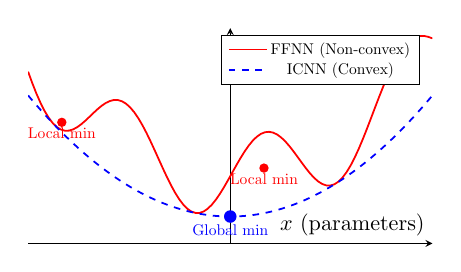
\begin{tikzpicture}[scale=0.8]
      \begin{axis}[
        width=8cm, height=5cm,
        axis lines=center,
        xlabel=$x$ (parameters), ylabel=Loss,
        xtick=\empty, ytick=\empty,
        ymin=0, ymax=8, xmin=-3, xmax=3,
        legend pos=north east,
        legend style={nodes={scale=0.7, transform shape}}
      ]
        \addplot[red, thick, domain=-3:3, samples=100]
          {0.5*x^2 + 1.5*sin(deg(3*x)) + 2.5};
        \addlegendentry{FFNN (Non-convex)}

        \addplot[blue, thick, dashed, domain=-3:3, samples=100]
          {0.5*x^2 + 1};
        \addlegendentry{ICNN (Convex)}

        \node[circle,fill=red,inner sep=1.5pt] at (axis cs:-2.5, 4.5) {};
        \node[red, below, scale=0.7] at (axis cs:-2.5, 4.5) {Local min};
        \node[circle,fill=red,inner sep=1.5pt] at (axis cs:0.5, 2.8) {};
        \node[red, below, scale=0.7] at (axis cs:0.5, 2.8) {Local min};

        \node[circle,fill=blue,inner sep=2pt] at (axis cs:0, 1) {};
        \node[blue, below, scale=0.7] at (axis cs:0, 0.9) {Global min};
      \end{axis}
    \end{tikzpicture}
  \end{column}
\end{columns}
\end{frame}

%---------------------------------------
\begin{frame}{What ICNN Buys for Macro Solvers}
\textit{\footnotesize Bellman equation stability and convergence.}
\begin{itemize}
  \item \textbf{Inner Bellman maximization is convex}: with a concave $V$ (or $-\text{ICNN}$), each $\max_{k'}\{u(k,k') + \beta\,\hat{V}(k')\}$ is a single-basin convex program
    \begin{itemize}
      \item Gradient / Newton methods land on the global maximum, every time
      \item No bracketing, no multi-start, no policy-iteration ``flips''
    \end{itemize}
  \medskip
  \item \textbf{Bellman operator remains a contraction}: ICNN preserves the shape required for $T$ to be a $\beta$-contraction on the value-function space
    \begin{itemize}
      \item VFI converges geometrically (same theoretical rate as classical VFI)
      \item Outer iterations are stable under repeated inner solves
    \end{itemize}
  \medskip
  \item \textbf{Equilibrium prices are well-behaved}: convex preferences $\Rightarrow$ monotone demand $\Rightarrow$ unique market-clearing prices in calibration loops
  \medskip
  \item \textbf{Cost paid}: a per-layer non-negativity reparameterization (Softplus) --- negligible at training time, large payoff in solver reliability
\end{itemize}
\end{frame}

%---------------------------------------
\begin{frame}[fragile]{ICNN: Robust PyTorch Implementation}
\textbf{Strategy}: Use reparameterization (Softplus) instead of clamping to enforce $W_z \geq 0$.
\vspace{-0.2cm}
\begin{lstlisting}[style=pythonstyle,basicstyle=\ttfamily\tiny]
class ICNN(nn.Module):
    def __init__(self, d_in, hidden_sizes):
        super().__init__()
        # Passthrough weights (Input -> Hidden) [unconstrained]
        self.W_x = nn.ParameterList([
            nn.Parameter(torch.randn(h, d_in))
            for h in hidden_sizes])
        # Recurrent weights (Hidden -> Hidden) [unconstrained params]
        # Apply Softplus() during forward pass to enforce W_z >= 0
        self.W_z_params = nn.ParameterList([
            nn.Parameter(torch.randn(h, h_prev))
            for h, h_prev in zip(hidden_sizes[1:], hidden_sizes[:-1])])
        self.biases = nn.ParameterList([
            nn.Parameter(torch.zeros(h)) for h in hidden_sizes])

    def forward(self, x):
        z = x
        for i, (Wz_p, Wx, b) in enumerate(
                zip(self.W_z_params, self.W_x, self.biases)):
            Wz = F.softplus(Wz_p)  # Enforce non-negativity
            z_next = F.linear(z, Wz) + F.linear(x, Wx) + b
            z = F.relu(z_next)
        return z
\end{lstlisting}
\end{frame}

%---------------------------------------
\begin{frame}{Monotonic NNs: Architecture --- Partial Monotonicity}
\textbf{Objective}: Ensure $f(x)$ is non-decreasing in (a designated subset of) inputs:
\[
  x_i \uparrow \;\Rightarrow\; f(x) \uparrow
\]

\vspace{0.1cm}
\textbf{Two necessary constraints}:
\begin{enumerate}
  \item \textbf{Non-negative weights}: $W^{(l)} \geq 0$ for all layers (biases unconstrained)
  \item \textbf{Monotonic activations}: $\sigma'(\cdot) \geq 0$ (ReLU, Sigmoid, Tanh, Softplus)
\end{enumerate}

\vspace{0.1cm}
\textbf{Enforcement} (same two methods as ICNN):
\begin{itemize}
  \item \textbf{Clamping}: simple, but pinned weights can kill neurons during training
  \item \textbf{Reparameterization (Softplus)}: preferred --- smooth gradients, well-conditioned
\end{itemize}

\vspace{0.1cm}
\textbf{Partial monotonicity}: split inputs into a ``monotone path'' (constrained weights) and a ``free path'' (unconstrained), then combine such that monotonicity in the designated inputs is preserved. The companion frame shows the propagation logic.
\end{frame}

%---------------------------------------
\begin{frame}{Monotonic NNs: Propagation Logic (visual)}
\begin{columns}
  \begin{column}{0.45\textwidth}
    \textbf{Why $x_i \uparrow \Rightarrow f(x) \uparrow$}:
    \begin{itemize}
      \item Input layer: $x$ enters with non-negative weights $W_1 \geq 0$
      \item Hidden activations $z$ inherit the increase
      \item Next layer: $W_2 \geq 0$ propagates the monotonicity again
      \item Monotonic $\sigma$ never flips signs
    \end{itemize}

    \vspace{0.15cm}
    \textbf{Failure modes if any condition slips}:
    \begin{itemize}
      \item Even one negative weight in the monotone path breaks the guarantee
      \item Non-monotone activation (e.g., GELU near zero) inverts gradients locally
    \end{itemize}
  \end{column}

  \begin{column}{0.55\textwidth}
    \centering
    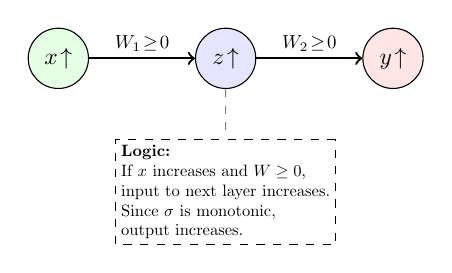
\begin{tikzpicture}[scale=0.85, transform shape,
      neuron/.style={circle, draw, minimum size=0.9cm},
      arrow/.style={->, thick}
    ]
      \node[neuron, fill=green!10] (I) at (0,0) {$x\!\uparrow$};
      \node[neuron, fill=blue!10] (H) at (2.5,0) {$z\!\uparrow$};
      \node[neuron, fill=red!10] (O) at (5,0) {$y\!\uparrow$};

      \draw[arrow] (I) -- (H) node[midway, above, scale=0.8] {$W_1 \!\geq\! 0$};
      \draw[arrow] (H) -- (O) node[midway, above, scale=0.8] {$W_2 \!\geq\! 0$};

      \node[draw, dashed, align=left, scale=0.7] at (2.5, -2) {
        \textbf{Logic:} \\
        If $x$ increases and $W \geq 0$, \\
        input to next layer increases.\\
        Since $\sigma$ is monotonic, \\
        output increases.
      };
      \draw[dashed, gray] (H) -- (2.5, -1.1);
    \end{tikzpicture}
  \end{column}
\end{columns}
\end{frame}

%---------------------------------------
\begin{frame}{Macro Application: Shape Restrictions on Policy Functions}
\begin{itemize}
\item \textbf{Economic theory pins down the sign of many partials}:
\begin{itemize}
    \item \textbf{Demand} non-increasing in price (law of demand)
    \item \textbf{Consumption} non-decreasing in wealth (normal goods)
    \item \textbf{Value functions} non-decreasing in the resource state
    \item \textbf{Savings policy} $a'(a,z)$ increasing in assets $a$
    \item \textbf{Wage curves} non-decreasing in productivity (or non-increasing in unemployment, depending on framing)
\end{itemize}

\medskip
\item \textbf{Use monotone networks to bake the theory in}:
\begin{itemize}
\item Savings rule monotone in $a$ but free in $z$ $\Rightarrow$ partial monotonicity (Aiyagari/Krusell--Smith setting, Lec06)
\item Consumption rule monotone in cash-on-hand $\Rightarrow$ avoids spurious wiggles common to FFNNs
\item Wage curve monotone in productivity $\Rightarrow$ stable labor-market mechanism
\end{itemize}

\medskip
\item \textbf{Bottom line}: monotone NNs guarantee economically sensible policies \emph{without post-hoc corrections}, and the validation gate becomes much sharper (Lab 3B's residual plot stops hiding shape violations)
\end{itemize}
\end{frame}

%---------------------------------------
\begin{frame}{Worked Example: Recovering Preferences via ICNN}
\textbf{Economic problem: Expenditure minimization}
\begin{align*}
  E(p, u) &= \min_{c \geq 0}\; p \cdot c \\
  \text{s.t.}\quad & U_\theta(c) \geq u \quad \text{(target utility)}
\end{align*}

\textbf{The ``structured'' solution}:
\begin{itemize}
  \item Learn the expenditure function $E_\theta(p, u)$ using a Concave ICNN
  \item \textbf{Theory}: the expenditure function $E(p, u)$ is concave in prices $p$ (a structural property of $E$)
\end{itemize}

\textbf{Why this is powerful}:
\begin{enumerate}
  \item \textbf{Shephard's Lemma + Auto-Diff}: $c^*(p, u) = \nabla_p E_\theta(p, u)$ --- demand functions for free!
  \item \textbf{Integrability}: Because $E_\theta$ is structurally concave, the resulting demands satisfy the Slutsky matrix properties by construction
\end{enumerate}

\vspace{0.1cm}
{\footnotesize\textit{The Shephard's Lemma example is the macroeconomist's first ICNN --- same architecture as Lec03 T4, named here for the economic content (cost minimization $\to$ conditional factor demands by partial derivatives).}}
\end{frame}

%---------------------------------------
\begin{frame}{Other Economic Applications}
\begin{itemize}
\item \textbf{ICNN for optimal transport / Wasserstein distance}:
\begin{itemize}
    \item Kantorovich duality: $W_1(\mu,\nu) = \sup_{f \text{ 1-Lipschitz}} \mathbb{E}_\mu[f] - \mathbb{E}_\nu[f]$
    \item ICNNs parameterize the convex conjugate --- used in generative models and distributional analysis
\end{itemize}

\medskip
\item \textbf{Concave value functions}:
\begin{itemize}
    \item In many macro models, $V(k)$ is concave in capital
    \item Approximate $V$ with $-\text{ICNN}(k)$ to enforce concavity \emph{by construction}
    \item Eliminates spurious non-concavities from unconstrained approximation
\end{itemize}

\medskip
\item \textbf{Structured value functions for HA models}:
\begin{itemize}
    \item In Krusell--Smith (Lecture 6), the policy function $a'(a, z; \Gamma)$ is monotone in $a$ and concave in cross-section
    \item Enforce both via PICNN with monotonicity constraint on $a$
\end{itemize}
\end{itemize}
\end{frame}

%---------------------------------------
\begin{frame}{Summary: Choosing the Right Architecture}
Don't use a black box when you have a blueprint.

\vspace{0.3cm}
\begin{table}[]
\centering
\renewcommand{\arraystretch}{1.4}
\small
\begin{tabular}{l | l | l}
\textbf{Economic Property} & \textbf{Architecture} & \textbf{Key Mechanism} \\
\hline
\textbf{Convexity} & ICNN & Non-neg weights + skip conn. \\
(Utility, costs) & & \\
\hline
\textbf{Partial Convexity} & Partial ICNN (PICNN) & Split paths (convex/free) \\
(Value functions) & & \\
\hline
\textbf{Monotonicity} & Monotonic NN & Non-neg weights \\
(Supply/demand) & Deep Lattice Nets & Interpolation \\
\hline
\textbf{Equilibrium} & Deep Equilibrium (DEQ) & Fixed point iteration \\
(Market clearing) & & \\
\end{tabular}
\end{table}

\vspace{0.2cm}
\textbf{Takeaway}: Imposing structure improves interpretability, sample efficiency, and ensures your model respects economic theory
\end{frame}

%=============================================================================
\section{Accuracy, Validation, and Lab Preview}

\sectiondivider{Accuracy, Validation, and Lab Preview}{Euler-residual audits and the Lab 3A/3B gate: never trust an unvalidated solution}

%---------------------------------------
\begin{frame}{Validation Philosophy: The Research Architect Approach}
\begin{itemize}
  \item In computational economics, getting code to \emph{run} is not enough
  \item The critical question: \textbf{Is the answer correct?}
  \medskip
  \item \textbf{Validation strategy} (used in Labs 6A and 6B):
    \begin{enumerate}
      \item Solve a model with a \textbf{known analytical solution} (log utility, Cobb-Douglas)
      \item Implement the numerical method
      \item Compare numerical output against the closed-form truth
      \item Report maximum absolute error across the state space
    \end{enumerate}
  \medskip
  \item \textbf{Key metrics}:
    \begin{itemize}
      \item Policy error: $\max_k |g_{\text{approx}}(k) - g^*(k)|$
      \item Value error: $\max_k |V_{\text{approx}}(k) - V^*(k)|$
      \item Euler equation error: $\max_k |\mathcal{R}(k; g_{\text{approx}})|$
    \end{itemize}
\end{itemize}
\end{frame}

%---------------------------------------
\begin{frame}{Euler Equation Error as a Diagnostic}
\begin{itemize}
  \item Even when no analytical solution exists, we can measure accuracy via the \textbf{Euler equation error}:
    \[
      EE(k) = \frac{u'(c)}{\beta\, \mathbb{E}[u'(c')\, f'(k')]} - 1
    \]
  \medskip
  \item \textbf{Interpretation}: $EE(k) = 0.01$ means the agent is making a 1\% optimization error at state $k$
  \medskip
  \item \textbf{Standard benchmarks} (Judd 1998):
    \begin{itemize}
      \item $\log_{10}|EE| < -3$: acceptable (error $< 0.1\%$)
      \item $\log_{10}|EE| < -5$: good (error $< 0.001\%$)
      \item $\log_{10}|EE| < -7$: excellent
    \end{itemize}
  \medskip
  \item This diagnostic works for \emph{any} model with Euler equations, not just those with analytical solutions
\end{itemize}
\end{frame}

%---------------------------------------
\begin{frame}{What Lab 3A Establishes: The Ground Truth}
\textbf{Lab 3A: Classical Benchmark (VFI)}
\begin{itemize}
  \item Solves the stochastic optimal growth model using VFI with interpolation
  \item Validates against the analytical solution ($c^* = (1-\alpha\beta)y$)
  \item Establishes the ``answer key'' for Lab 3B
\end{itemize}

\vspace{0.2cm}
\textbf{Key takeaways from Lab 3A}:
\begin{enumerate}
  \item The benchmark exists: we know \emph{exactly} what the optimal policy looks like
  \item VFI works, but requires a grid --- breaks in high dimensions
  \item The 5-step Research Architect workflow:
    \begin{enumerate}
      \item Mathematical formulation (Bellman equation)
      \item Algorithmic specification (VFI with interpolation)
      \item Define deliverables (class structure, plots, errors)
      \item AI-augmented implementation (structured prompting)
      \item Critical validation (numerical vs.\ analytical)
    \end{enumerate}
\end{enumerate}
\end{frame}

%---------------------------------------
\begin{frame}{What Lab 3B Demonstrates: Neural Network Solutions}
\textbf{Lab 3B: Two Deep Learning Approaches}

\vspace{0.15cm}
\textbf{Part 1: Deep Value Function Iteration}
\begin{itemize}\footnotesize
  \item Two networks (\texttt{PolicyNet} + \texttt{ValueNet}) with $T$-step lookahead and soft constraints
  \item \textbf{Pros}: provides both policy and value; handles inequality constraints naturally
  \item \textbf{Cons}: slower convergence; more hyperparameters
  \item Validated: savings rate $k'/y$ converges to $\alpha\beta$
\end{itemize}

\vspace{0.1cm}
\textbf{Part 2: Euler Equation Minimization}
\begin{itemize}\footnotesize
  \item Train a \texttt{PolicyNetwork} with constrained output to minimize Euler residual
  \item \textbf{Pros}: very precise policy; theoretically grounded
  \item \textbf{Cons}: no value function; requires deriving FOCs
  \item Validated against analytical policy $k'^* = \alpha\beta\, y$
\end{itemize}

\vspace{0.1cm}
\begin{tcolorbox}[colback=blue!3, colframe=blue!40, fontupper=\scriptsize, boxsep=2pt, top=2pt, bottom=2pt,
                   title={\scriptsize Lab 3A $\to$ 3B handshake}]
Lab 3A produces ground truth via classical VFI on a fine grid. Lab 3B trains the NN. The Euler-residual heatmap (T3) is the validation gate: if the NN's residual is within $10^{-3}$ of the Lab 3A solution on a held-out test grid, it passes.
\end{tcolorbox}
\end{frame}

%---------------------------------------
\begin{frame}{Lab Preview: What You Will Do}
\textbf{Lab 3A: The Classical Benchmark} (VFI)
\begin{itemize}
  \item Build an \texttt{OptimalGrowthModel} class in Python
  \item Implement VFI with \texttt{scipy.interpolate} and \texttt{scipy.optimize}
  \item Validate against the analytical solution
  \item \textbf{Notebook}: \texttt{Lab3A\_Dynamic\_Models.ipynb}
\end{itemize}

\vspace{0.3cm}
\textbf{Lab 3B: Neural Network Solutions} (PyTorch)
\begin{itemize}
  \item Part 1: Train a DVFI solver with $T$-step lookahead and soft constraints
  \item Part 2: Train an Euler equation solver --- compare against Lab 3A's ground truth
  \item Compare convergence speed, accuracy, and which method yields richer output
  \item \textbf{Notebook}: \texttt{Lab3B\_Dynamic\_Models.ipynb}
\end{itemize}

\vspace{0.3cm}
\textbf{Goal}: Experience the full pipeline from classical methods to deep learning, using the same model throughout for direct comparison

\vspace{0.2cm}
{\footnotesize \emph{For a full treatment of classical VFI, interpolation, and perturbation methods, see the video series at \url{https://space.bilibili.com/2142649036/lists/7180709}.}}
\end{frame}


%=============================================================================
% BRIDGE TO LEC06
%=============================================================================

\begin{frame}{Lecture 4, Complete: One Map, Four Acts}
\textbf{You solved one model four ways --- exactly, on a grid, by actor--critic, and by Euler residuals --- and audited every neural answer against ground truth.}

\LecFourMap{0}

\vspace{0.05cm}
\footnotesize\textit{Keep the pattern: pose the model, choose the loss (Bellman or Euler), train, then \emph{validate before you trust}. Lec.\ 5 supplies the RL theory we previewed; Lec.\ 6 runs this pipeline on heterogeneous-agent models.}
\end{frame}

\begin{frame}{Preview: What Lec.\ 5 \& Lec.\ 6 Deliver}
\begin{itemize}
  \item \textbf{Next --- Lec05 (Reinforcement Learning in a Nutshell):} the general framework behind the actor-critic we \emph{previewed} in T2--T3.
    \begin{itemize}
      \item \textbf{T1} --- RL framework \& the dynamic-programming connection (Bellman, back to Lec01).
      \item \textbf{T2} --- tabular methods: Monte Carlo, TD(0), Q-learning, SARSA.
      \item \textbf{T3} --- actor-critic as an \emph{algorithm family} (policy-gradient theorem; A2C / PPO / DDPG / SAC) + applications.
    \end{itemize}
  \medskip
  \item \textbf{Then --- Lec06 (Heterogeneous-Agent Models via RL):} the \emph{same} audit gates (Lab 3A ground truth, Lab 3B NN solution, Euler-residual heatmap) reused on much harder state spaces --- Aiyagari / Krusell--Smith / DeepHAM, Deep Equilibrium Nets (DEQN), OLG, and mean-field games.
\end{itemize}

\vspace{0.2cm}
\textit{The validation discipline you learned here is the bridge: Lec05 gives you the RL theory, Lec06 puts it to work on the cross-sectional distribution.}
\end{frame}

%=============================================================================
% SUMMARY
%=============================================================================

\begin{frame}{Summary}
\begin{enumerate}
  \item \textbf{The problem}: Grid-based methods break due to the curse of dimensionality
  \medskip
  \item \textbf{The opportunity}: Neural networks are universal approximators that scale polynomially, not exponentially, with dimension
  \medskip
  \item \textbf{Two approaches}:
    \begin{itemize}
      \item \textbf{Actor-Critic / DVFI}: Two networks approximate $V(k)$ and $g(k)$; RL flavor
      \item \textbf{Euler Equation}: One network minimizes the Euler residual; supervised learning flavor
    \end{itemize}
  \medskip
  \item \textbf{Structured networks} (ICNN, MNN) embed economic theory into the architecture, ensuring well-behaved solutions
  \medskip
  \item \textbf{Validation}: Always compare against known analytical solutions or Euler equation errors
  \medskip
  \item \textbf{Next:} Lec.\ 5 develops the RL framework behind actor-critic in depth; Lec.\ 6 scales the validation discipline to heterogeneous-agent models
\end{enumerate}
\end{frame}

\end{document}
